\subsection{digitales Theremin}\label{subsec:Theremin_digital}

Wie schon am Anfang dieses Kapitels angedeutet, werden in diesem zweiten Teil Möglichkeiten für den Aufbau des Theremins als ein digitales Instrument aufgezeigt.
\begin{figure}[h]
	\centering
	\includegraphics[width=0.7\textwidth]{Blockschaltbild_digital.pdf}
	\caption{Blockschaltbild digitales Theremin mit eingezeichneten Ausgängen.}
	\label{img:Blockschaltbild_digital}
\end{figure}

\paragraph{Antennenoszillator}\mbox{}\\
\\Um den Oszillator zur Änderung der Tonhöhe und der Lautstärke zu realisieren waren mehrere Optionen möglich. Diese wurden in der Projektklärung genauer verglichen (siehe Anhang). Schlussendlich wurde entschieden, dass dieser Teil des Theremins weiterhin analog bleiben soll, um das Theremin wie anhin spielen zu können, ohne einen extremen Aufwand treiben zu müssen. Das generierte Signal wird an \textit{osc\_out} ausgegeben.

\paragraph{Referenzoszillator}\mbox{}\\
\\Der zweite Oszillator wird nun digital realisiert. Dazu wurden zwei Möglichkeiten in Erwägung gezogen. Zum einen ein Oszillator mithilfe von Lookup Tables. Diese brauchen keine komplizierte Berechnung sondern nur eine Tabelle mit den Sinuswerten einer viertel Periode. Diese würden dann so ausgegeben, dass eine ganze Periode entsteht. Die zweite und etwas aufwendigere Variante ist ein Sinusgenerator mithilfe des Cordic Algorithmus. Bei diesem werden die Werte erst während der Laufzeit berechnet. Dazu wird zum einen eine Komponente benötigt, welche den Sinus Wert berechnet und zum anderen eine Komponente welche die entsprechenden Winkelwerte in der richtigen Frequenz bereitstellt.

Es wurde entschieden den Cordic Algorithmus einzusetzen, da dieser zeitgemässer ist und einen grösseren Lerngewinn bietet.

Der Cordic Algorithmus wird gebraucht, um verschiedenste mathematische Operationen iterativ grösstenteils nur mit Additionen und Verschiebung von Bits zu berechnen. Im Falle des Theremins wurde dieser gebraucht, um aus einem vorgegebenen Winkel den Sinus zu berechnen.
Der Cordic Algorithmus kann in zwei Modi betrieben werden. Zum einen der Vektor Modus, mit welchem von einem gegebenen Vektor der Winkel berechnen werden kann und zum anderen der Rotationsmodus, mit welchem aus einem gegebenen Winkel die Elemente des zugehörigen Vektors berechnet werden können. Für die beiden Modi werden folgende Formeln verwendet \cite{Cordic}:

\begin{equation}
x_{i+1} = x_i - y_id_i2^{-i}
\label{equ:cordic_1}
\end{equation} 
\begin{equation}
y_{i+1} = y_i + x_id_i2^{-i}
\label{equ:cordic_2}
\end{equation} 
\begin{equation}
z_{i+1} = z_i - d_i\arctan{2^{-i}}
\label{equ:cordic_3}
\end{equation} 

Dabei wird \(d_i\) im Rotationsmodus wie folgt berechnet: 

\begin{equation}
d_i=
\begin{cases}
     -1 &z_i < 0 \\
     1 &\text{otherwise}
\end{cases}
\label{equ:cordic_4}
\end{equation} 

Wie man sieht werden in jeder Iteration die neuen Werte aus den alten Werten berechnet. Um den Algorithmus so einzusetzen, dass aus einem gegebenen Winkel der Sinus und der Kosinus berechnet wird, müssen die benötigten Anfangsbedingungen wie folgt gewählt werden:
\begin{equation}
\begin{aligned}
x_0 = 1 \\
y_0 = 0 \\
z_0 = \varphi
\end{aligned}
\label{equ:cordic_3}
\end{equation} 

\(\varphi\) ist der gegebene Winkel, welcher zwischen \(-\pi/2\) und \(\pi/2\) sein muss, damit der Algorithmus konvergiert.

Daraus ergeben sich nach \(n\) Iterationen der Sinus und Kosinus Wert wie folgt:

\begin{equation}
\begin{aligned}
x_n = \frac{\cos{\varphi}}{A} \\
y_n = \frac{\sin{\varphi}}{A}
\end{aligned}
\label{equ:cordic_3}
\end{equation} 

Somit müssen am Schluss noch die erhaltenen Werte mit der Konstante \(A = 0.60725294\) multipliziert werden um die genauen Sinus- und Kosinuswerte zu erhalten. Diese Resultate werden am Ausgang \textit{ref\_out} ausgegeben.



\paragraph{Mischer}\mbox{}\\
\\Der Mischer kann als digitale Komponente sehr einfach realisiert werden. Er muss lediglich die beiden Signale der Oszillatoren \textit{osc\_out} und \textit{ref\_out} miteinander multiplizieren. Weiter wurde das Signal \textit{osc\_out} in ein Rechtecksignal gewandelt. Dies ermöglicht es auf einen Analog-Digital-Wandler zu verzichten. Dies ändert nichts an der Funktionalität des Theremins, da die Oberwellen des Rechtecksignals eine so hohe Frequenz haben, dass sie nie in die nähe der hörbaren Frequenzen kommen. Auch nach dem mischen haben die Produkte zwischen Referenzoszillator und Oberwellen noch so hohe Frequenzen, dass dies keine Probleme bereitet. Das gemischte Resultat wird am Ausgang \textit{mix\_out} ausgegeben.
\clearpage
\paragraph{Tiefpassfilter}\mbox{}\\

\begin{figure}[h]
\centering
\includegraphics[width=\textwidth]{CIC_Filter.pdf}
\caption{Aufbau eines CIC-Filters N-ter Ordnung mit Eingang mix\_out und Ausgang filt\_out}
\label{img:CIC_Filter}
\end{figure}
Um das gemischte Signal am Ende mit einem Tiefpass zu filtern, sind verschiedene Methoden möglich. Zum einen können FIR oder IIR Filter eingesetzt werden. Da das Signal am Ende unterabgetastet werden muss, um die richtige Frequenz für den Digital-Analog-Wandler zu erhalten, war die Verwendung eines CIC-Filters ideal. Dieses hat zudem den Vorteil, dass keine Multiplikationen durchgeführt werden müssen, da es lediglich Additionen und Subtraktionen benötigt \cite{cic_h}.


Wie man in Abbildung \ref{img:CIC_Filter} sieht ist das Filter in drei Stufen aufgeteilt. Die erste Stufe bildet der Integratorfilter, welcher alle Eingangswerte aus \textit{mix\_out} aufsummiert. Dabei ist der entstehende wrap-araound durchaus gewünscht. In der zweiten Stufe wird die Abtastrate \(fs\) des Signals um den Faktor \(R\) dezimiert. Die dritte Stufe enthält den Combfilter, welcher mit einer tieferen Abtastrate die Daten verarbeitet. Dabei wird der aktuelle Abtastwert mit dem letzten subtrahiert und an \textit{filt\_out} ausgegeben.
Zudem können mehrere Integrator- und Combfilterpaare hintereinandergeschalten werden um die Ordnung des Filters zu erhöhen. Dieses Filter hat im Vergleich zur normalen Unterabtastung weniger Aliasing zur Folge \cite{cic_a}.





\paragraph{Digital-Analog-Wandler}\mbox{}\\
\\Um die diskreten Daten als Ton auszugeben wird ein Digital-Analog-Wandler (DAC) benötigt. Damit der DAC korrekt funktioniert, müssen die Daten an \textit{filt\_out} mit einer bestimmten Abtastfrequenz zur Verfügung gestellt werden. Das analoge Signal wird an \textit{dac\_out} an den Lautsprecher ausgegeben.


